\section{La transformada discreta de Fourier y estudios espectrales de señales finitas}

\TODO{aquí una introducción}
\TODO{La teoría se basa en el libro de Algoritmos.}

La teoría de esta sección se apoya en la existencia de las raíces
$n-$ésimas de la unidad (garantizada por el teorema fundamental
del álgebra \ref{teo: fundamental del algebra}) 
y propiedades de estas que hacen posible
tener un método eficiente de calcular lo que después llamaremos
la ``transformada discreta'' de un elemento de $\IC^{n}$.

\subsection{Raíces $n-$ésimas de la unidad y propiedades de estas}

\TODO{Habla sobre la exponencial compleja; tal vez pon su definición,
pero di que no entras en detalles (estos pueden consultarse, por ejemplo, en Marsden), sólo citamos unas propiedades de esta función de $\IC$ a $\IC$
que necesitaremos}

\TODO{Tal vez puedes hablar de cómo esta forma involucra al ángulo y
a la norma para representar a un punto, y por qué esto es útil
para hablar de mulitplicación y conjugados! También tienes que definir
la norma en $\IC^{n}$, esto no es trivial y de hecho me estaba dando
problemas.}

\begin{prop}
\label{prop: propiedades exp compleja}
(\textbf{Propiedades de la exponencial compleja}) a
	\begin{itemize}
	\item $exp(z) = 1$ si y sólo si $z= 2K \pi i$ para algún $K \in \IZ$
	\item Para todo $\omega \in \IZ$ y todo $z \in \IC$, $(exp(z))^{\omega} = 			exp(\omega z)$ \TODO{ve si $\omega$ puede de hecho ser cualquier complejo? 			tiene sentido esto?}
	\item Para cualesquiera $z_{1}, z_{2} \in \IC$, 
	$\frac{exp(z_{1})}{exp(z_{2})} = exp(z_{1} - z_{2})$.
	\item Para todo entero $n$ y todo real $b$,
	$(exp(bi))^{m} = exp (mb i)$
	\item \TODO{pon lo de exponencial de la suma.}
	\end{itemize}
\end{prop}


\begin{defi}
\label{defi: raices n esimas de la unidad}
Sea $n \in \IN$. A las $n$ raíces del polinomio
$p_{n}(t)= t^{n}-1$ se les denominará las \textbf{raíces $n-$ésimas de la unidad.}
\end{defi}


Las raíces $n-$ésimas de la unidad son pues los números complejos
tales que, elevados a la potencia $n$, son iguales a 1; según el 
teorema fundamental
del álgebra \ref{teo: fundamental del algebra}, sí hay números complejos
que satisfacen la definición \ref{defi: raices n esimas de la unidad}, y además
son a lo más $n$. Es fácil establecer, como hacemos a continuación, 
fórmulas explícitas para estos números, que de hecho son exactamente $n$.

\begin{prop}
Sea $n \in \IN$, $n \geq 2$. Hay exactamente $n$ raíces $n-$ésimas de la
unidad, y estas son los números complejos
 	\begin{equation}
	\label{eq3: 8ab}
	z_{n, \omega} : = exp \left( \frac{2 \pi i }{n} \omega
	\right), \hspace*{0.2cm} \textit{con} 
	\hspace*{0.2cm} \omega \in \{0, 1, \ldots, n-1 \}.
	\end{equation}
	
\end{prop}
\noindent
\textbf{Demostración.}
Por las propiedades expresadas en la proposición
\ref{prop: propiedades exp compleja}, es fácil ver que 
$z_{n,1} :=  exp \left( \frac{2 \pi i }{n} \right)$ es raíz $n-$ésima
de la unidad, pues
\[
(z_{n,1})^{n} = exp(2 \pi i ) = 1.
\]
Además, para todo $\omega \in \{ 0, \cdots , n-1 \}$, el número
\[
z_{n, \omega} : = (z_{n,1})^{\omega} = exp \left( \frac{2 \pi i }{n} \omega \right)
\]
también es es raíz $n-$ésima de la unidad, ya que

\[
(z_{n, \omega})^{n} = ((z_{n,1})^{\omega} )^{n} = 
((z_{n,1})^{n} )^{\omega} = 1^{\omega}=1. 
\]
Note ahora que los $n$ números complejos $z_{n, \omega}$ son todos 
distintos entre sí, pues si $\omega_{1}$ y $\omega_{2}$ son enteros
entre $0$ y $n-1$ tales que $z_{n, \omega_{1}} = z_{n, \omega_{2}}$,
o sea, tales que 
$exp \left( \frac{2 \pi i }{n} \omega_{1} \right) = 
exp \left( \frac{2 \pi i }{n} \omega_{1} \right)$, entonces, según el tercer
punto de la proposición \ref{prop: propiedades exp compleja},
$1 = exp \left( \frac{2 \pi i }{n} (\omega_{1}-\omega_{2}) \right)$, luego, 
según el primer punto de esta misma proposición, $\frac{\omega_{1}-\omega_{2}}{n}$
es entero, o sea, $n$ divide a $\omega_{1}-\omega_{2}$; por el rango de 
$\omega_{1}$ y $\omega_{2}$, esto sólo ocurre si $\omega_{1}-\omega_{2}$ es
cero, o sea, si $\omega_{1}$ y $\omega_{2}$
son iguales.
\QEDB
\vspace{0.2cm}

\TODO{Aquí la figura de siempre:)}



\subsection{DFT}




\begin{prop}
Sea $n \in \IN$. El conjunto

\begin{equation}
\label{eq2: 8ab}
\cali{B}_{n} : = \{
e_{\omega} = \left(
\frac{1}{\sqrt{n}} exp \left(
2 \pi i \omega \frac{m}{n}
\right)
\right)_{0 \leq m \leq n-1}
: \hspace{0.2cm} 0 \leq \omega \leq n-1
 \}
\end{equation}
es una base ortonormal del $\IC-$espacio
vectorial $\IC^{n}$.
\end{prop}

\noindent
\textbf{Demostración.}
Calculemos el producto punto de dos elementos
$e_{\omega_{1}}$ y $e_{\omega_{2}}$ del conjunto \eqref{eq2: 8ab};
si $\omega := \omega_{1}-\omega_{2}$,
\begin{align*}
\langle e_{w_{1}}, e_{w_{2}} \rangle = &
\frac{1}{n}
\suma{m=0}{n-1}{exp \left( 2 \pi i \frac{m}{n} \omega_{1} \right)
\cdot \overline{ exp \left( 2 \pi i \frac{m}{n} \omega_{2} \right) }} \\
= & \frac{1}{n}
\suma{m=0}{n-1}{\left( 2 \pi i \frac{m}{n} (\omega_{1}-\omega_{2}) \right)} \\
= & \frac{1}{n}\suma{m=0}{n-1}{exp\left( 2 \pi i \frac{\omega}{n} m \right)} \\
= & \frac{1}{n}\suma{m=0}{n-1}{exp\left( 2 \pi i \frac{\omega}{n}  \right)^{m}} \\
= & \frac{1}{n}\suma{m=0}{n-1}{(z_{n, \omega})^{m}};
\end{align*}

\noindent
esta última es una suma geométrica. 
\begin{itemize}
	\item Si $\omega_{1} \neq \omega_{2}$, entonces $n$ no puede dividir 
	a $\omega = \omega_{1}-\omega_{2}$ (pues, por el rango en el que se encuentran
	$\omega_{1}$ y $\omega_{2}$, $w \in [-(n-1), n-1]$, y el único múltiplo
	de $n$ en este intervalo es cero), luego, $z_{n, \omega} \neq 1$.
	En este caso se tiene entonces que 
	\[
	\langle e_{w_{1}}, e_{w_{2}} \rangle = 
	\frac{1}{n}\suma{m=0}{n-1}{(z_{n, \omega})^{m}}
	= \frac{1}{n} \cdot \frac{(z_{n, \omega})^{n}-1}{z_{n, \omega}-1}=
	\frac{1}{n} \cdot \frac{1-1}{z_{n, \omega}-1}=0.
	\]
	
	\item Si $\omega_{1} = \omega_{2}$, entonces $\omega = 0$, y
	\[
	\langle e_{w_{1}}, e_{w_{2}} \rangle = 
	\frac{1}{n}\suma{m=0}{n-1}{(z_{n, 0})^{m}}
	= \frac{1}{n}\suma{m=0}{n-1}{1} = \frac{1}{n} \cdot n = 1.
	\]
\end{itemize}

Demostramos así que los elementos de $\cali{B}_{n}$
tienen norma uno (c.f. \TODO{ref ec. norma en $\IC^{n}$}) y que además
son ortogonales
dos a dos, luego, según \TODO{ref}, $\cali{B}_{n}$ es un subconjunto l.i. 
de $\IC^{n}$; como $\IC^{n}$ es un $\IC-$espacio vectorial de 
dimensión $n$, concluimos lo deseado.
\QEDB
\vspace{0.2cm}

Por ser \eqref{eq2: 8ab} una BON de $\IC^{n}$, siempre es
posible expresar a un vector $x = (x_{m})_{0 \leq m \leq n-1} \in \IC^{n}$
como combinación lineal de los elementos de \eqref{eq2: 8ab}
y además los coeficientes están dados por los productos puntos
de $x$ y los elementos de \eqref{eq2: 8ab}, que son

\begin{align*}
\langle x, e_{\omega} \rangle = & 
\frac{1}{\sqrt{n}} \suma{m=0}{n-1}{x_{m} exp \left(
2 \pi i \omega \frac{m}{n}
\right)} \\
= & 
\frac{1}{\sqrt{n}} \suma{m=0}{n-1}{x_{m} 
\left(
exp \left( \frac{2 \pi i }{n} \omega
\right) \right)^{m}} \\
= & A_{x}(z_{n, \omega}),
\end{align*}


\noindent
donde $z_{n, \omega}$ es como en \eqref{eq3: 8ab} y 
$A_{x} = A_{x}(t) \in \IC[t]$ es el polinomio de 
coeficientes complejos definido 
a partir de $x$ como sigue:

	\begin{equation}
		\label{eq4: 8ab}
		A_{x}(t) := \suma{m=0}{n-1}{\frac{x_{m}}{\sqrt{n}} t }\in \IC[t];
	\end{equation}

\noindent
así, \textbf{calcular los coeficientes de $x \in \IC^{n}$ respecto
a la BON $\cali{B}_{n}$ es lo mismo que evaluar al polinomio 
$A_{x}$ de grado $n-1$ definido en \eqref{eq4: 8ab} en todas las raíces
$n-$ésimas de la unidad.} Un algoritmo para evaluar eficientemente
polinomios es pues necesario.\TODO{cita el FFT}

\begin{defi}
Al proceso de calcular los coeficientes de $x$
respecto a $\cali{B}_{n}$
se le conoce como el \textbf{cálculo de la 
transformada discreta de $x$}
\end{defi}


\begin{comment}
{\Huge{\textcolor{red}{TDF}}} 

{\Huge{\textcolor{red}{Dominio: tiempo}}} 


{\Huge{\textcolor{red}{Dominio: frecuencia}}}

{\Huge{ $x = (x_{m})_{0 \leq m \leq n-1}$ }}

{\Huge{ $\langle x, e_{\omega} \rangle$, $0 \leq \omega \leq n-1 $ }}

\end{comment}


\begin{figure}[H]
\centering\captionsetup{format = hang}
	\begin{measuredfigure}
		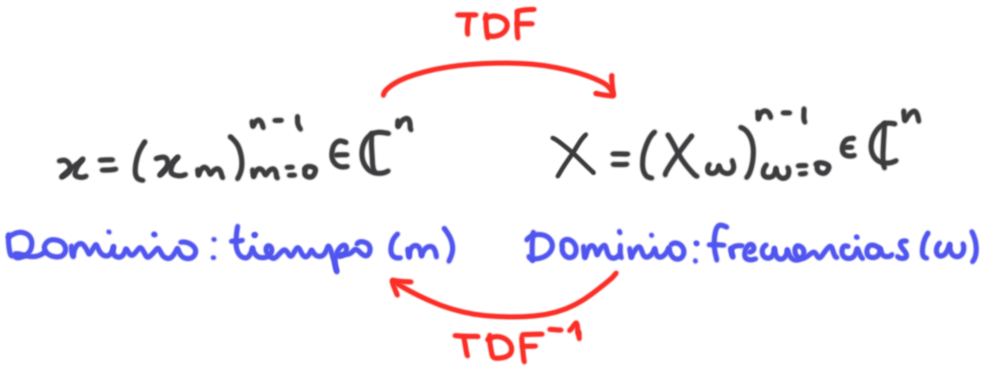
\includegraphics[scale=0.8]{tiempo_freq.png} 
		\caption{Usualmente uno representa a una señal discreta
		$x$ de dimensión $n$ con $n$ mediciones complejas; en este caso, el dominio
		de la representación es el tiempo. Pero, según lo explicado,
		también se puede representar unívocamente a $x$ con sus
		coeficientes respecto a la base de frecuencias 
		$\cali{B}_{n}$; en este caso, puesto que cada coeficiente da
		el peso que tiene la respectiva frecuencia para construir la 
		señal original $x$, decimos que el dominio de la representación
		es el de frecuencia.}
 	\end{measuredfigure}
 \end{figure}


Al usar a $\cali{B}_{n}$ como sistema de representación en
$\IC^{n}$, lo que estamos haciendo es representar a
un $x = (x_{m})_{0 \leq m \leq n-1}$ como combinación
lineal de los vectores 

\[
e_{\omega} = \frac{1}{\sqrt{n}} \left( cos
\left( 2 \pi \omega \frac{m}{n} \right)
+ i sen \left( 2 \pi \omega \frac{m}{n}\right) \right)_{0\leq m \leq n-1},
\hspace{0.2cm} 0 \leq \omega \leq n-1;
\]
observe que las partes reales de las
entradas de $e_{\omega} \in \IC^{n}$ se obtienen de tomar $n$
muestras uniformes de la función 
$c_{\omega}(t) := \frac{1}{\sqrt{n}} cos (2 \pi \omega t)$ (o sea, de la función
coseno de amplitud $\frac{1}{\sqrt{n}}$, frecuencia $\omega$ y desfase $0$)
y, similarmente,
las partes imaginarias de las entradas se obtienen muestreando
uniformemente a la función 
$s_{\omega}(t) := \frac{1}{\sqrt{n}}  sin (2 \pi \omega t)$.

\TODO{En los vectores $e_{\omega}$ deberías poner la dependencia
a la dimensión $n$...}

\begin{figure}[H]
	\sidecaption{
	Por ejemplo, si $n=5$, para construir al vector
	$e_{3}$ de la base $\cali{B}_{n}$ se muestrean uniformemente
	cosenos y senos de frecuencia $3$ como se muestra en la figura;
	los puntos rojos representan las partes reales de las entradas
	y los azules las imaginarias.
	\label{fig: construccion Bn}
	}
	\centering
	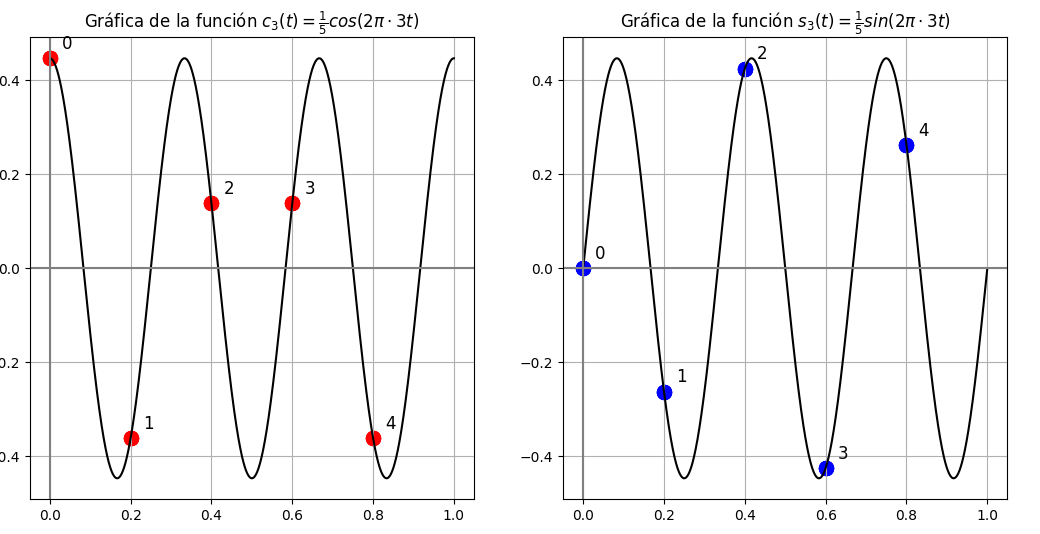
\includegraphics[scale=0.44]{construccion_Bn} 
\end{figure}	

Según esto, el vector $e_{\omega}$ se construye a partir
de funciones de frecuencia $\omega$; considerando esto
y el que $\cali{B}_{n}$ sea una BON de $\IC^{n}$ (luego, el
que se valga la igualdad de Parseval \TODO{ref}), tenemos que
la síntesis

\[
x = \suma{\omega=0}{n-1}{\langle x, e_{\omega} \rangle e_{\omega}}
\]

es una expresión de $x$ en términos de vectores de frecuencia
$\omega$ y que los respectivos coeficientes 
$\langle x, e_{\omega} \rangle$ indican qué tanto 
contribuye la frecuencia $\omega$ para construir a $x$.

Es por eso que al proceso de considerar representaciones
de señales complejas finitas respecto a las bases de Fourie
se le conoce como  
\textbf{realizar un análisis espectral.}


\subsection{Versión real de la DFT}

En el caso en el que todas las entradas de un vector
$x = (x_{m})_{0 \leq m \leq n-1}$ sean reales, se puede definir
una base ortonormal de $\IR^{n}$ que se defina en base a muestreos uniformes
de sinusoides de frecuencias enteras.
Esta base será entonces, así como lo era \TODO{ref} para el 
caso complejo, un sistema de representación en el que 

\TODO{sintetizar una señal en términos de frecuencias.}

\begin{prop}
\label{prop: base de fourier version real}
Sean $n \in \IN$ mayor a uno, $M = \lceil \frac{n}{2} \rceil$.
Para cualquier $\omega >0$, sean los vectores 

	\begin{equation}
	\label{eq0: 10ab}
	c_{n, \omega} := \left( \sqrt{\frac{2}{n}} cos
	\left(2 \pi \omega \frac{m}{n}
	\right) \right)_{0 \leq m \leq n-1}
	\hspace{0.2cm} \textit{y} \hspace{0.2cm} 
	s_{n, \omega} := \left( \sqrt{\frac{2}{n}} sin
	\left(2 \pi \omega \frac{m}{n}
	\right) \right)_{0 \leq m \leq n-1}.
	\end{equation}

El subconjunto $\cali{F}_{n}$ de $\IR^{n}$ definido como

	\begin{itemize}
	\item $\cali{F}_{n} : = \{ c_{n,0}, c_{n,1}, s_{n,1},
	\ldots , c_{n,M-1}, s_{n,M-1}, c_{n,M} \}$ si $n$ es par
	(o sea, si $n=2M$), y como
	\item $\cali{F}_{n} : = \{ c_{n,0}, c_{n,1}, s_{n,1},
	\ldots , c_{n,M-1}, s_{n,M-1} \}$ si $n$ es impar
	(o sea, si $n=2M-1$)
	\end{itemize}
	
es una base ortonormal del $\IR-$espacio vectorial $\IR^{n}$.
\end{prop}

\noindent
\textbf{Demostración.}
Supongamos $n$ par. Si $0 \leq \omega_{1}, \omega_{2} \leq M$
son enteros, entonces
$\omega_{1} + \omega_{2}$ sólo es divisible por $n$ si ambos números
son iguales a $M$. Si suponemos a $\omega_{1}$ y $\omega_{2}$ distintos, 
entonces

\begin{align*}
\langle c_{, \omega_{1}} , c_{n, \omega_{2}} \rangle = &
\frac{1}{n} \suma{m=0}{n-1}{cos \left(2 \pi \omega_{1} \frac{m}{n} \right) \cdot 
cos \left(2 \pi \omega_{2} \frac{m}{n} \right)} \\
= &\frac{1}{2n} \left(
cos \left(2 \pi (\omega_{1} + \omega_{2}) \frac{m}{n} \right) +
cos \left(2 \pi (\omega_{1} - \omega_{2}) \frac{m}{n} \right)
\right) \\
= & \frac{1}{4n} (
\suma{m=0}{n-1}{
(exp(2 \pi m(\omega_{1}+\omega_{2})i/n) +
exp(-2 \pi m(\omega_{1}+\omega_{2})i) } \\
&  + exp(2 \pi m(\omega_{1}-\omega_{2})i/n) +
exp(-2 \pi m(\omega_{1}-\omega_{2})i)) )\\
\textit{(suma geométrica)} = & 
\frac{exp(2 \pi i (\omega_{1}+\omega_{2}))-1}{4n (exp(2 \pi i (\omega_{1}+\omega_{2})/n)-1)} +
\frac{exp(- 2 \pi i (\omega_{1}+\omega_{2}))-1}{4n (exp(-2 \pi i (\omega_{1}+\omega_{2})/n)-1)}
\\
& + 
\frac{exp(2 \pi i (\omega_{1}-\omega_{2}))-1}{4n (exp(2 \pi i (\omega_{1}-\omega_{2})/n)-1)} +
\frac{exp(- 2 \pi i (\omega_{1}-\omega_{2}))-1}{4n (exp(-2 \pi i (\omega_{1}-\omega_{2})/n)-1)};
\\
\end{align*}

\noindent
puesto que $\omega_{1}+\omega_{2}$ y $\omega_{1}-\omega_{2}$
son ambos enteros, según la proposición 
\ref{prop: propiedades exp compleja} las exponenciales de los numeradores
de esta última expresión son todas iguales a uno, luego, 
$\langle c_{n, \omega_{1}} , c_{n, \omega_{2}} \rangle  =0$. 


Con argumentos similares se prueba 
que todos los elementos de $\cali{F}_{n}$ tienen norma uno, así como
la ortogonalidad entre dos elementos
distintos del conjunto $\cali{F}_{n}$, por lo tanto, la independencia lineal de
este conjunto, luego, el que $\cali{F}_{n}$ sea base 
(ortonormal) de $\IR^{n}$.


\QEDB
\vspace{0.2cm}



\begin{defi}
Sea $n \in \IN$, $n \geq 2$. Llamaremos a la BON
$\cali{F}_{n}$ de $\IR^{n}$ definida en \ref{prop: base de fourier version real}
la \textbf{base de Fourier real de dimensión $n$}.
\end{defi}

Observe que $\cali{F}_{n}$, a diferencia de $\cali{B}_{n} \subseteq \IC^{n}$, 
considera frecuencias enteras no mayores a $M := \lceil \frac{n}{2} \rceil$
(cuando $n$ es par) o a $M-1$ (cuando $n$ es impar), mientras que
en $\cali{B}_{n}$ se consideran las frecuencias enteras entre $0$
y $n-1$ (inclusivo). Es decir, si 
\TODO{vamos a sintentizar a una señal respecto a menos frecuencias enteras.} 



\textbf{Ejemplo:} Consideremos a la señal 
\begin{equation}
\label{eq2: 10ab}
x=(-0.5,-8,-5.3,15,-0.3,6,4) \in \IR^{7}.
\end{equation}

Según la construcción de $\cali{F}_{7}$ (c.f. 
proposición \ref{prop: base de fourier version real}),
una expresión de $x$ respecto a $\cali{F}_{7}$ 
es una síntesis de $x$ a partir de señales 
de frecuencias $\omega = 0,1,2,3$. En la imágen de abajo
se muestran los coeficientes de $x$ respecto a $\cali{F}_{7}$.

\begin{figure}[H]
	\sidecaption{
	Se muestran la gráfica de $x$ junto con la gráfica de los
	coeficientes de $x$ respecto a la BON $\cali{F}_{7}$. Observe 
	que, por definición, sólo un vector de $\cali{F}_{7}$ tiene frecuencia
	cero (i.e. es constante), mientras que para las otras frecuencias
	tenemos dos vectores de la misma frecuencia, uno construido a partir de un 			coseno y otro a partir de un seno.
	\label{fig: ejFrecuencia 1}
	}
	\centering
	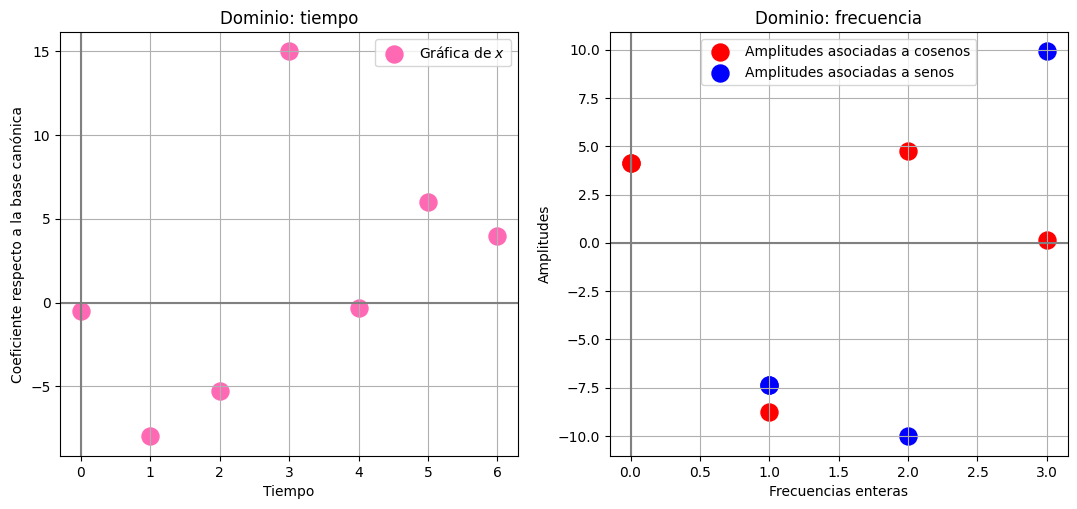
\includegraphics[scale=0.4]{ejFrecuencia_1} 
\end{figure}	

Se tiene la siguiente descomposición
\sidenote{Se redondearon los coeficientes.} de $x$;

\[
x = 4.12 c_{0} - 8.76c_{1} -7.35s_{1}+
4.77c_{2}-10s_{2}+0.14c_{3}+9.91s_{3}.
\]
A continuación mostramos las gráficas
de los sinusoides que fueron discretizados
para obtener los vectores de frecuencia
$0,1,2$ y $3$ en los que descompusimos a $x$.

\begin{figure}[H]
	\sidecaption{
	Aporte de frecuencia $0$.
	\label{fig: ejFrecuencia 2}
	}
	\centering
	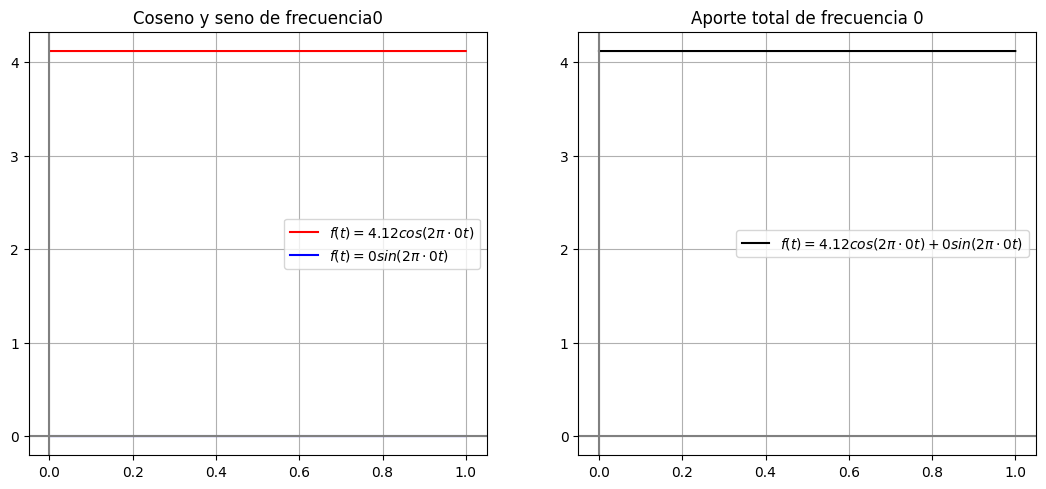
\includegraphics[scale=0.4]{ejFrecuencia_2} 
\end{figure}	

\begin{figure}[H]
	\sidecaption{
	Aporte de frecuencia $1$.
	\label{fig: ejFrecuencia 3}
	}
	\centering
	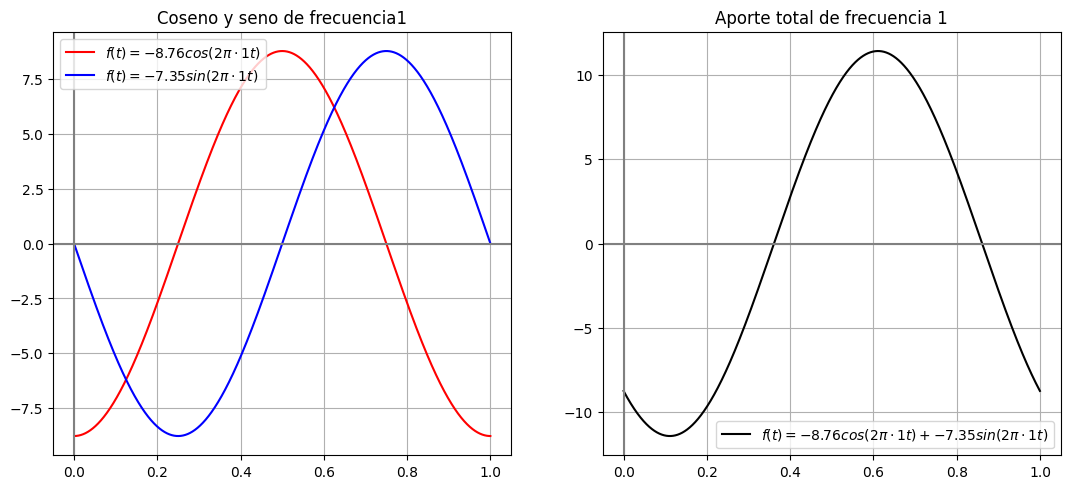
\includegraphics[scale=0.4]{ejFrecuencia_3} 
\end{figure}	

\begin{figure}[H]
	\sidecaption{
	Aporte de frecuencia $2$.
	\label{fig: ejFrecuencia 4}
	}
	\centering
	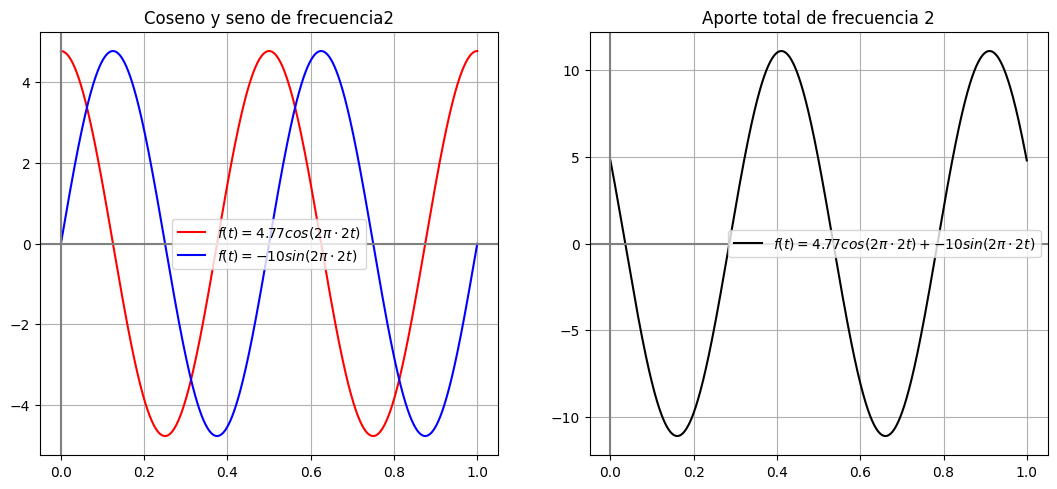
\includegraphics[scale=0.4]{ejFrecuencia_4} 
\end{figure}	


\begin{figure}[H]
	\sidecaption{
	Aporte de frecuencia $3$.
	\label{fig: ejFrecuencia 5}
	}
	\centering
	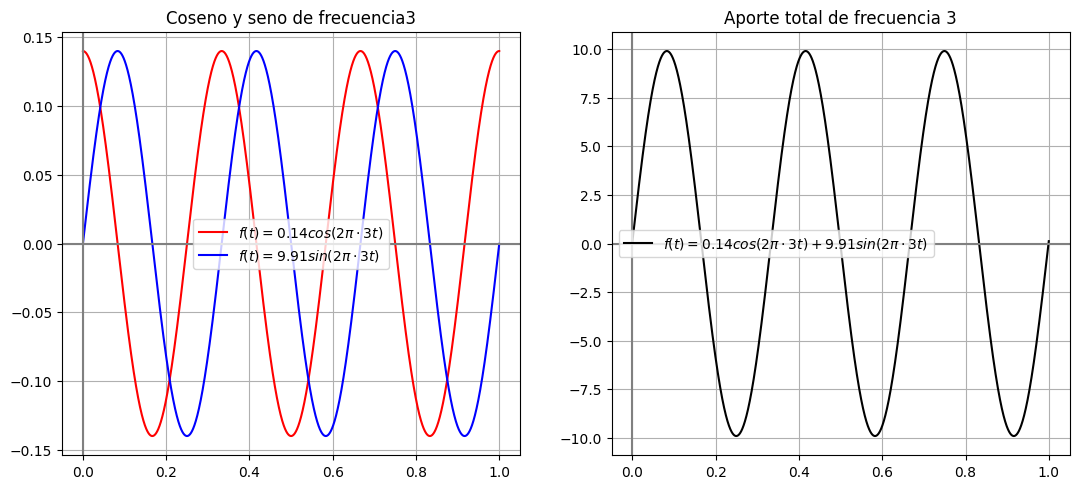
\includegraphics[scale=0.4]{ejFrecuencia_5} 
\end{figure}	

Sumando todas las gráficas de la derecha, obviamente
obtenemos una función de cosenos y senos tal que,
al muestrearla uniformemente en $[0,1]$, obtenemos
al vector $x$ \eqref{eq2: 10ab}.

\begin{figure}[H]
	\sidecaption{
	En morado se muestra la gráfica de la función suma
	de las gráficas derechas en las figuras anteriores.
	\label{fig: ejFrecuencia 6}
	}
	\centering
	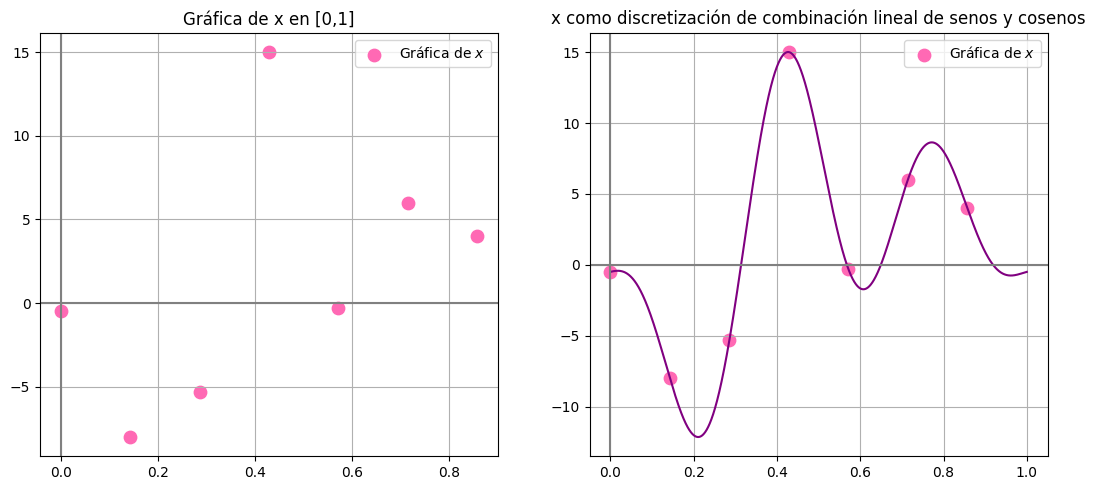
\includegraphics[scale=0.44]{ejFrecuencia_6} 
\end{figure}	


\TODO{Tal vez el algoritmos de la FFT no merezca una subsección. Mejor sólo 
exboza los detalles y cite al libro.}
\TODO{Para esto puedes apoyarte mucho en las notas del libro 
de Algorithms. Eso sí lo entendí bien.}




















